\section{Conversion of transformations}


In this section, we present the conversion of a transformation of the voxel space into a transformation of the world space, and conversely. We first introduce in Fig.~\ref{fig:tools:conv:1} a scheme that will be useful to give an intuition of how the conversion procedure works. This array visually represent the projection of a point from one image to another one, or from coordinate system to another one. On the top are represented the fixed and the moving images and on the left hand-side are represented the voxel and the world coordinate systems. We present here two arrows representing the projection of a point from the voxel coordinates to the world coordinates (see Section~\ref{subsec:images:systems:projection}). In this section, $M_{fixed}$ and $M_{moving}$  will respectively represent the projection (4$\times$4) matrix of the fixed and moving images.

\begin{figure}[!htbp]
\centering
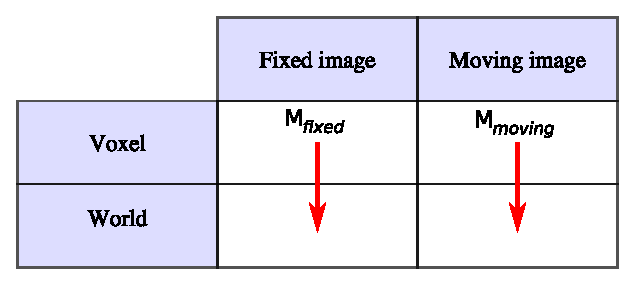
\includegraphics[width=0.5\linewidth]{conversion_transform1}
\caption{Projection matrices from the voxel coordinates to the world coordinates.}
\label{fig:tools:conv:1}
\end{figure}



%----------------------------------------------------------------------------------------------------
\subsection{Linear transformation: from voxel to world coordinates}

Let $T_{voxel}$ be a linear transformation (4$\times$4 matrix) from the fixed image to the moving image and given in the voxel coordinates (see Fig.~\ref{fig:tools:conv:2}). The conversion of $T_{voxel}$ into $T_{world}$, the corresponding linear transformation in the world coordinates, is given by:
%
\begin{equation}
T_{world} = M_{moving} . T_{voxel} . M^{-1}_{fixed}
\label{eq:tools:conv1}
\end{equation}
%
Fig.~\ref{fig:tools:conv:3} gives a visual explanation of the conversion. This conversion is used in the registration method Baloo where the initial code returns a linear transformation such as $T_{voxel}$. In the original version of Baladin, the returned transformation $T_{voxel}$ is a linear transformation from the moving image to the fixed image and given in the voxel coordinates. In this particular case, $T_{voxel}$ must be inverted before computing $T_{world}$ (from fixed to moving image) as proposed in Eq.~\ref{eq:tools:conv1}.
\\
From Eq.~\ref{eq:tools:conv1} one trivially converts a linear transformation from world coordinates to voxel coordinates:
%
\begin{equation}
T_{voxel} = M^{-1}_{moving} . T_{world} . M_{fixed}
\label{eq:tools:conv2}
\end{equation}
%
In the case of Baladin, the final transformation $T_{voxel}$ since Baladin consider transformations from the moving image to the fixed image.

\begin{figure}[!htbp]
\centering
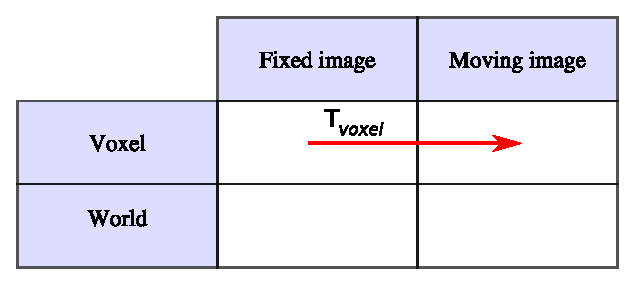
\includegraphics[width=0.5\linewidth]{conversion_transform2}
\caption{Transformation from the fixed image to the moving image and given in the voxel coordinates.}
\label{fig:tools:conv:2}
\end{figure}

\begin{figure}[!htbp]
\centering
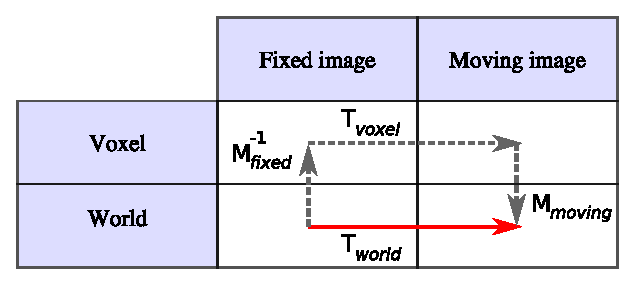
\includegraphics[width=0.5\linewidth]{conversion_transform3}
\caption{Conversion procedure: from voxel to world coordinates.}
\label{fig:tools:conv:3}
\end{figure}



%----------------------------------------------------------------------------------------------------
\subsection{Displacement field: from voxel to world coordinates}

The conversion of a displacement field is different from the conversion of a linear transformation. Indeed, a displacement vector is assigned to each element of the field. Let $p_{voxel}$ be an index of the fixed image (point in the voxel coordinates) and let $v_{voxel}$ be its associated displacement vector given in voxels. Let $p_1$ be the projection of $p_{voxel}$ into the world coordinates:
%
\begin{equation}
p_1 = M_{fixed} . p_{voxel}
\end{equation}
%
By definition, $p_{voxel} + v_{voxel}$ is an index in the moving image (point in the voxel coordinates). Let be $p_2$ be the projection of $p_{voxel} + v_{voxel}$ into the world coordinates:
%
\begin{equation}
p_2 = M_{moving} . \left( p_{voxel} + v_{voxel} \right)
\end{equation}
%
Both $p_1$ and $p_2$ are points in the world coordinates. The displacement vector, denoted $v_{world}$, in the world coordinates corresponding to $v_{voxel}$ is simply the difference between $p_2$ and $p_1$ (see Fig.~\ref{fig:tools:conv:4}):

%
\begin{equation}
v_{world} = M_{moving} . \left( p_{voxel} + v_{voxel} \right) - M_{fixed} . p_{voxel}
\end{equation}
%

\begin{figure}[!htbp]
\centering
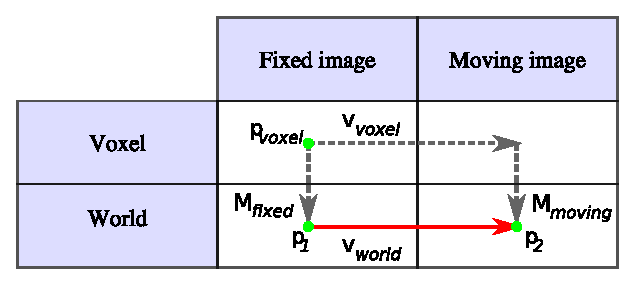
\includegraphics[width=0.5\linewidth]{conversion_transform4}
\caption{Conversion of a displacement field from voxel to world coordinates. Green circles represent (from top to bottom and left to right) $p_{voxel}$, $p_1$, and $p_2$.}
\label{fig:tools:conv:4}
\end{figure}